\documentclass[12pt, a4paper]{article}
\usepackage{amsfonts, amsmath, amsthm}
\usepackage[utf8x]{inputenc}
\usepackage{indentfirst}
\usepackage{multirow}
\usepackage[table]{xcolor}
\usepackage{listings}
\usepackage{alltt}
\usepackage{fancyvrb}
\usepackage{amsmath}
\usepackage{graphicx}
\usepackage{algorithm}
\usepackage{algpseudocode}
\usepackage{subfigure}
\usepackage{setspace}
\usepackage{wrapfig}
\usepackage{colortbl}
\usepackage{wrapfig}
\usepackage{tikz}
\usepackage{subfig}
\usepackage[hyphens]{url}
\usepackage{setspace}


\usetikzlibrary{positioning}
\graphicspath{ {./images/} }


\title{%
	
\includegraphics[height=0.3\textwidth]{UNITBV2.png}~ 
	\\[1cm]
	\vspace{20mm}
	
	\bf 	LUCRARE DE LICENȚĂ
	\noindent\rule{14cm}{1pt}
	\bf Serenity Garden TD
}

\onehalfspacing

\date{}

\begin{document}
	
	
	
	\maketitle
	\vspace{10mm} %5mm vertical space
	\begin{flushleft}
		\bf 	Conducător Stiintific:
		\bf     \\Lector Universitar Deaconu Adrian
	\end{flushleft}
	
	\begin{flushright}
		\bf Absolvent:
		\bf \\Opria Ion-Bogdan
	\end{flushright}
	
	\vspace{6mm} %5mm vertical space
	
	\begin{center}
		\bf Brașov, 2021 
	\end{center}
	
	
	\tableofcontents
	\pagebreak
	
	\section{Introducere}
	
	\subsection{Descrierea proiectului}
	
	Jocurile video au inceput sa acapareze din ce in ce mai mult vietile noastre datorita usurintei de accesare si a experientei pe care o ofera. Odata cu evolutia hardware-ului, jocurile video au devenit din ce in ce mai realiste si prin urmare ofera experiente care nu poat fi gasite in niciun alt mediu existent, deoarece in nici un alt mediu nu putem controla si traii experientele unor caractere atat de indetaliat. Industria jocurilor video este o industrie care este in continua crestere si prin urmare este o ramura care merita explorata din perspectiva unui programator si nu nu mai. 
	
	"Games are great to work on because they are as much about art as they are science." \cite{gameProgrammingComplete}
	
	Din aceste motive, am ales drept proiect pentru licenta sa fac un joc video. Jocul se numeste "Serenity Garden" si este un tower defense 3D. Experienta jocului are loc in cateva nivele special definite, in care utilizatorul trebuie sa isi protejeze baza de operatii. Exista multe tipuri diferite de inamici care vor sa distruga baza jucatorului, iar acesta, pentru a o proteja, trebuie sa construiasca un sistem defensiv. Jucatorul poate sa construiasca turnuri defensive care au diferite efecte asupra inamicilor. Inamicii ataca sistemul defensiv, sau in cazul in care lipseste, ataca direct baza jucatorului. Daca reusesc sa distruga baza, jucatorului, acesta pierde nivelul curent.
	
	Jucatorul nu poate sa construiasca turnuri oriunde, ci are locuri predefinite unde poate sa le construiasca, locuri specificate de hexagoane colorate pe harta de joc. Odata plasat un turn, aceasta nu poate fi mutat, dar jucatorul are si un caracter invulnerabil pe care il poate muta oriunde doreste pe harta. Acest caracter va ataca inamicii automat cand nu se afla in miscare, si poate intra in turnuri pentru a le creste puterea/eficienta.
	
	Modul care va diferentia acest joc de celelalte jocuri pe acest stil este modul de co-op. Doi jucatori se vor putea conecta prin retea si vor juca un nivel dificil care necesita cooperare si o planificare buna intre ei.
	
	\subsection{Introducere in dezvoltarea jocurilor video}
	
	\subsubsection{Scurta istorie}
	
	\subsubsection{Industria curenta}
	
	
	
	\section{Introducere in Unity}
	
	\subsection{Prezentare generala}
	
	
	\subsubsection{GameObject si Mesh}
	
	\subsubsection{Collider}
	
	\subsubsection{Transform si Rigidbody}
	
	\subsubsection{API-ul de scriptare}
	
	\subsection{Motivul alegerii pentru proiectul de licenta}

	\subsection{Elemente specifice folosite}	
	
	\subsubsection{Shader Graph}
	
	\subsubsection{VFX Graph}
	
	\subsubsection{Photon Engine}
	
	
	
	\section{Planificare Proiect}
	
	\subsection{Faza de Proiectare}
	
	"Almost anything that you can be good at can become a useful
	skill for a game designer." \cite{bookOfLenses}
	
	Din proiecte precedente am realizat ca o planificare buna a unui proiect inca de la inceput poate imbunatatii calitatea proiectului explonential, asigura usurinta de adaugare a unor elemente noi (fara sa fie necesara rescrierea/reorganizarea proiectului) si reduce frustrarea programatorilor care lucreaza la proiect.
	
	Din acest motiv, inca de la inceputul proiectului am incercat sa imi planific cat mai indetaliat continutul acestuia si modul in care il voi implementa.
	
	In prima faza, mi-am scris un document de proiectare care continea descrierea si elementele jocului, privite din multe perspective.
	
	Introducerea proiectului a fost realizata la inceputul acestui document si nu va fi reluata aici.
	
	
	
	\subsection{Tematica Jocului}
	
	Jocul are loc in viitorul departat. Planeta ta este supra-populata, iar nivelul de poluare a ajuns la un nivel critic. Umanitatea a trecut de mult de punctul in care mai pot salva aceasta planeta. Intreaga planeta va deceda in cateva decenii, iar oamenii daca nu isi gasesc o alta locuinta intre timp, vor muri si ei impreuna cu ea. In acest scop, o armata speciala a fost formata, care are ca scop explorarea altor planete si gasirea uneia care poate suporta rasa umana.
	
	Universul este totusi foarte periculos. Unele planete au viata extraterestra foarte agresiva, iar altele au fost distruse de experimente cibernetice esuate. Jucatorul este comandantul suprem al acestei armate care are ca scop protejarea oamenilor de stiinta care vor analiza aceste planete.
	
	Prima faza a proiectului va contine o singura planeta care poate fi populata dar care contine multi inamici periculosi.
	
	Planeta mama trimite resurse din cand in cand, dar numai un numar limitat de resurse pot fi trimise deodata, iar acestea dureaza mult timp sa ajunga, asa ca nu putem depinde de ele in timpul unei lupte.
	
	
	
	\subsection{Caracterele Jocului}
	
	\textbf{Comandantul} este protagonistul jocului. El este caracterul a carei perspective o vom traii pe tot parcursul jocului. In trecut a fost cobai pentru un experiment menit sa creeze super-soldati, iar in urma acestui experiment a primit o putere speciala. Poate sa isi ascunda complet prezenta fata de alti oameni sau alte creaturi. Din acest motiv, el este caracterul invulnerabil pe care il putem misca pe harta in timpul luptei.
	
	
	
	\subsubsection{Inamicii}
	\begin{itemize}
		\item \textbf{Inamicul de lupta apropiata} este un tip de inamic care poate ataca turnurile doar cand sta fix in fata lor. Are viata mai multa decat inamicii de lupta de la distanta.
		\item \textbf{Inamicul de lupta de la distanta} este un tip de inamic care poate ataca turnurile de la distanta. Are viata putina, dar pot ataca repede.
		\item \textbf{Inamicul zburator} este un inamic care poate fi lovit doar de un numar limitat de turnuri.
		\item \textbf{Inamicul bombardier} este un tip de inamic care ignora turnurile intalnite in cale. Acesta se misca pe cel mai scurt drum catre baza jucatorului, iar daca ajunge deasupra acesteia, va lansa bombe care ii vor scadea drastic viata, dupa care vor pleca de pe mapa. Este un tip de inamic zburator care poate fi lovit doar de un numar limitat de turnuri.
	\end{itemize}

	Acesti inamici (cu exceptia bombardierului) se vor misca pe harta calculand cel mai scurt drum catre baza jucatorului. Daca acestia intalnesc in cale un turn, se vor opri si vor ataca acel turn. Cand turnul este distrus, acestia isi vor relua drumul.
	
	Pentru fiecare inamic vor fi 3 tipuri de variatii, fiecare mai puternic decat cel precedent.
	
	
	
	\subsubsection{Turnuri defensive}
	In continuare voi scrie o descriere scurta pentru fiecare turn din joc. Toate proprietatile despre care urmeaza sa vorbesc sunt in comparatie cu celelalte turnuri defensive.
	\begin{itemize}
		\item \textbf{Serenity} este baza jucatorului. Are viata foarte multa daca este distrusa jucatorul pierde nivelul curent. Aceasta poate ataca inamicii care se apropie de ea. Are raza de atac medie, putere de atac mediu, poate ataca orice tip de inamic, iar rata de reincarcare intre atacuri este mica (dureaza mult timp intre atacuri)
		\item \textbf{Mitraliera automata} (fig: \ref{fig: machineGun}) Are viata mica, poate ataca orice tip de inamic, are raza medie, putere de atac mica si rata de atac este mare (ataca foarte des)
		\item \textbf{Gardul electric} (fig: \ref{fig: electricFence}) este turnul de protectie. Are viata foarte mare, poate ataca doar inamicii de lupta apropiata, puterea de atac este medie, iar rata de reincarcare este mica. Scopul acestui turn este sa stea in calea inamicilor pentru a fi atacat de acestia, permitand celorlalte turnuri sa atace inamicii blocati.
		\item \textbf{Vulkan} (fig: \ref{fig: vulkan}) Este turnul special construit pentru a lupta impotriva inamicilor zburatori. Are viata putina, raza de atac mare si putere de atac mare dar poate ataca doar inamicii zburatori.
		\item \textbf{Aruncatorul de flacari} (fig: \ref{fig: machineCannon}). Cand inamicii intra in raza acestui turn, el va imprastia flacari catre inamici. Toti inamicii care intra in aceste flacari primesc damage in fiecare clipa in care stau in flacari. Are viata medie, ataca instant si puterea de atac este mica dar distribuita in fiecare clipa in care inamicii stau in flacarile acestui turn.
		\item \textbf{Laser} (fig: \ref{fig: railgun}). Este un turn similar cu aruncatorul de flacari in sensul in care ataca in fiecare clipa in care un inamic este in raza acestuia. Ataca cu un laser puternic care scade treptat viata inamicilor. Are viata medie, ataca instant si puterea de atac este mica.
		\item \textbf{Excavator} (fig: \ref{fig: excavator}) este un tip special de turn deoarece nu poate ataca inamicii. Acesta aduna resurse in timpul luptei, resurse care pot fi convertite in bani de joc. Are viata multa, si pentru ca nu poate ataca, trebuie sa fie aparat de inamici.
	\end{itemize}
	
	
	\begin{figure}[H]
		\centering
		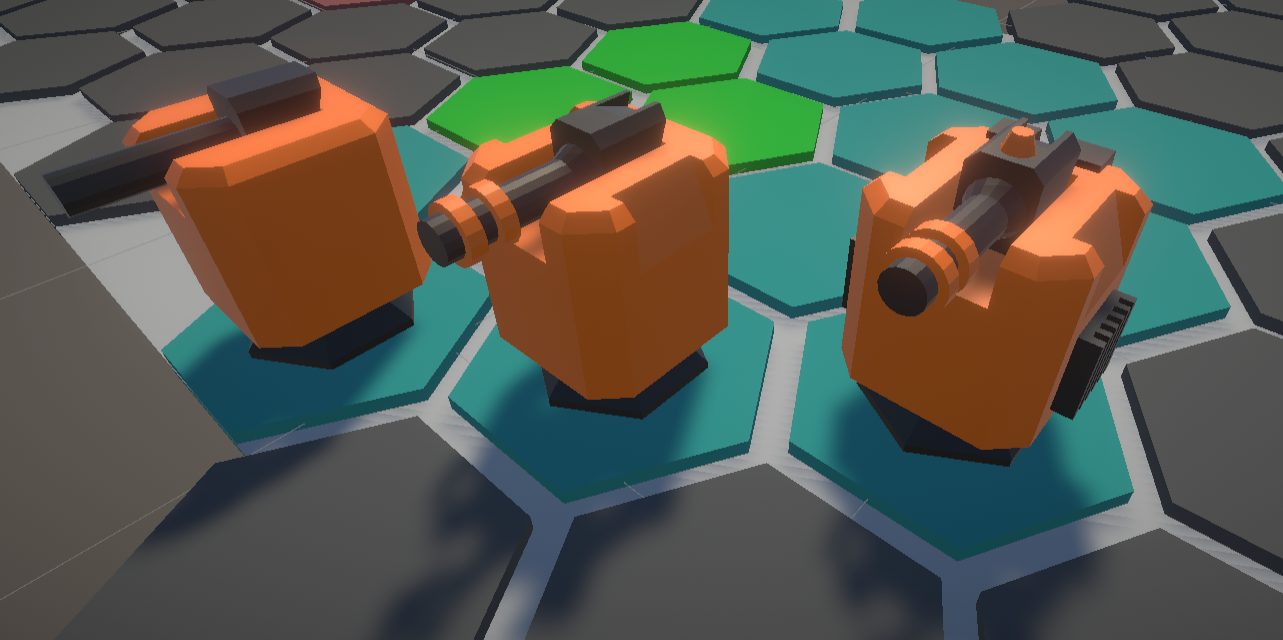
\includegraphics[width=1\textwidth]{machineGun.png}
		\caption{Mitraliera automata}
		\label{fig: machineGun}
	\end{figure}

	\begin{figure}[H]
		\centering
		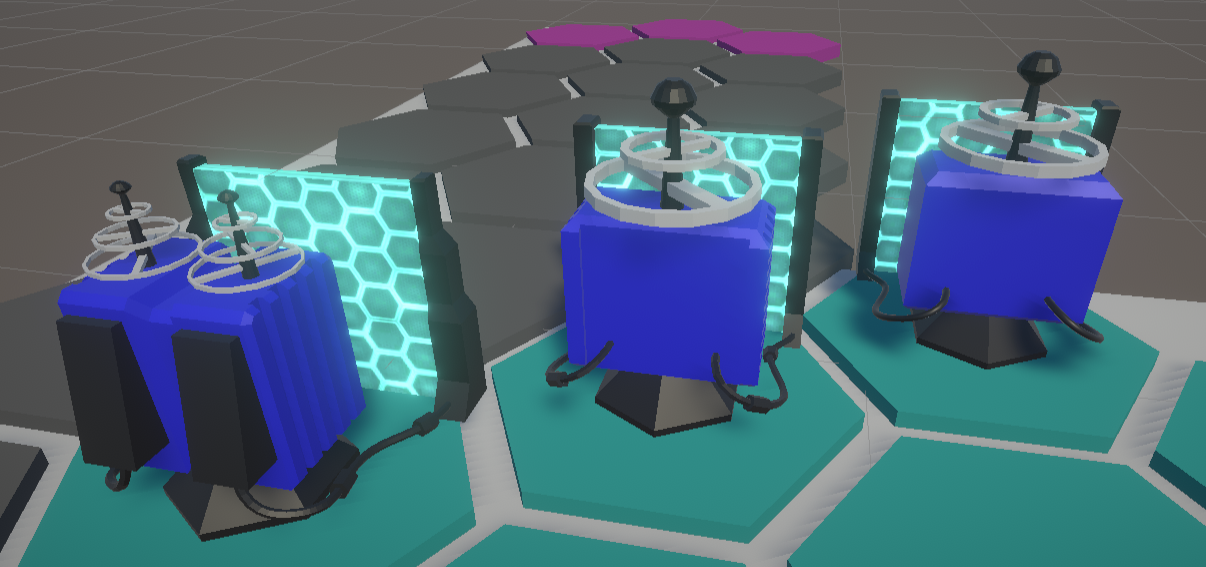
\includegraphics[width=1\textwidth]{electricFence.png}
		\caption{Gardul electric}
		\label{fig: electricFence}
	\end{figure}

	\begin{figure}[H]
		\centering
		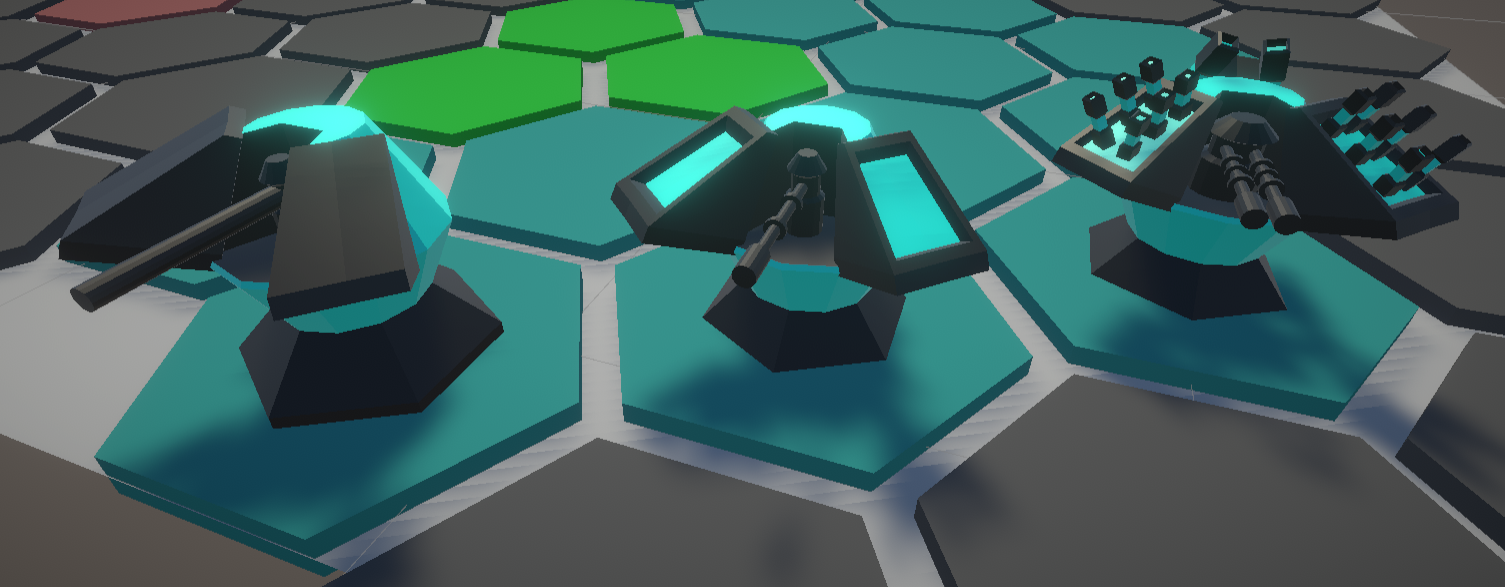
\includegraphics[width=1\textwidth]{vulkan.png}
		\caption{Vulkan}
		\label{fig: vulkan}
	\end{figure}

	\begin{figure}[H]
		\centering
		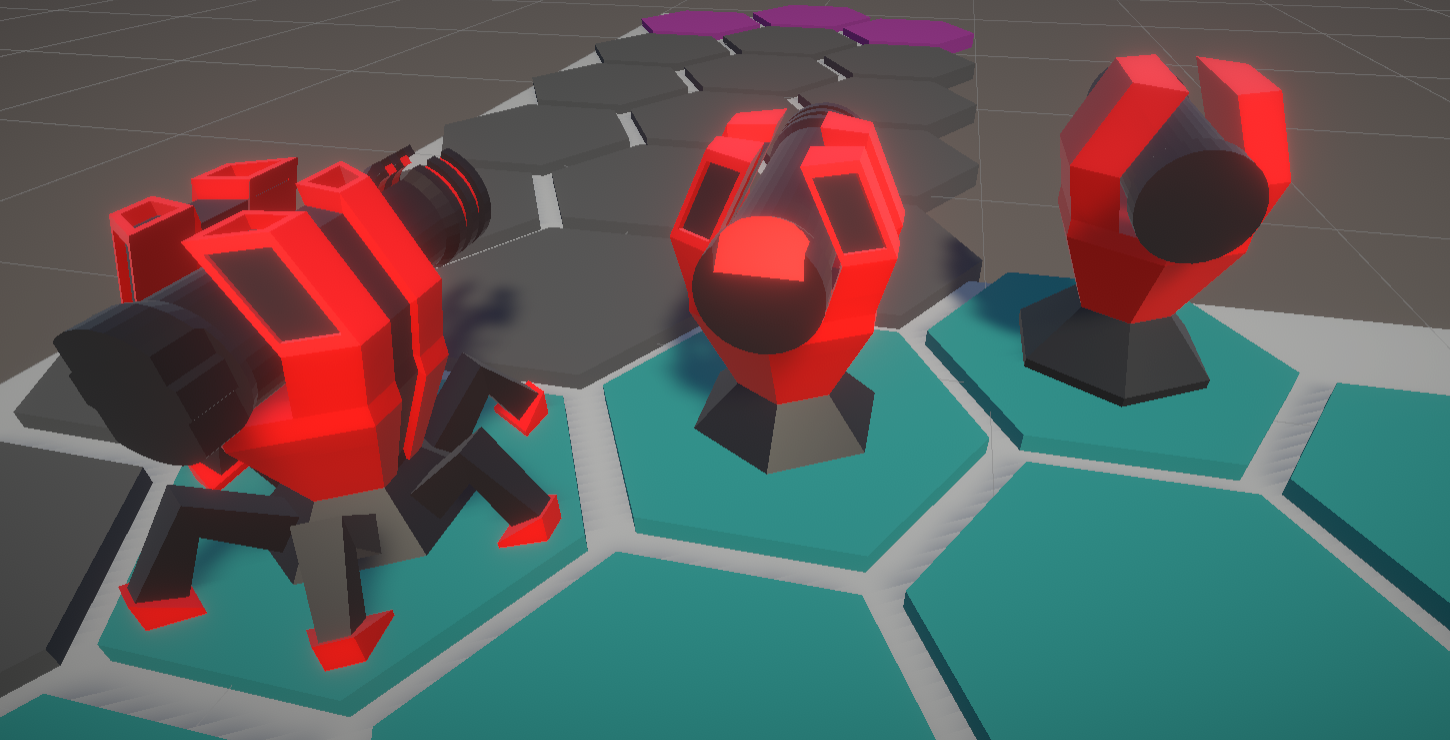
\includegraphics[width=1\textwidth]{machineCannon.png}
		\caption{Aruncatorul de flacari}
		\label{fig: machineCannon}
	\end{figure}
	
	\begin{figure}[H]
		\centering
		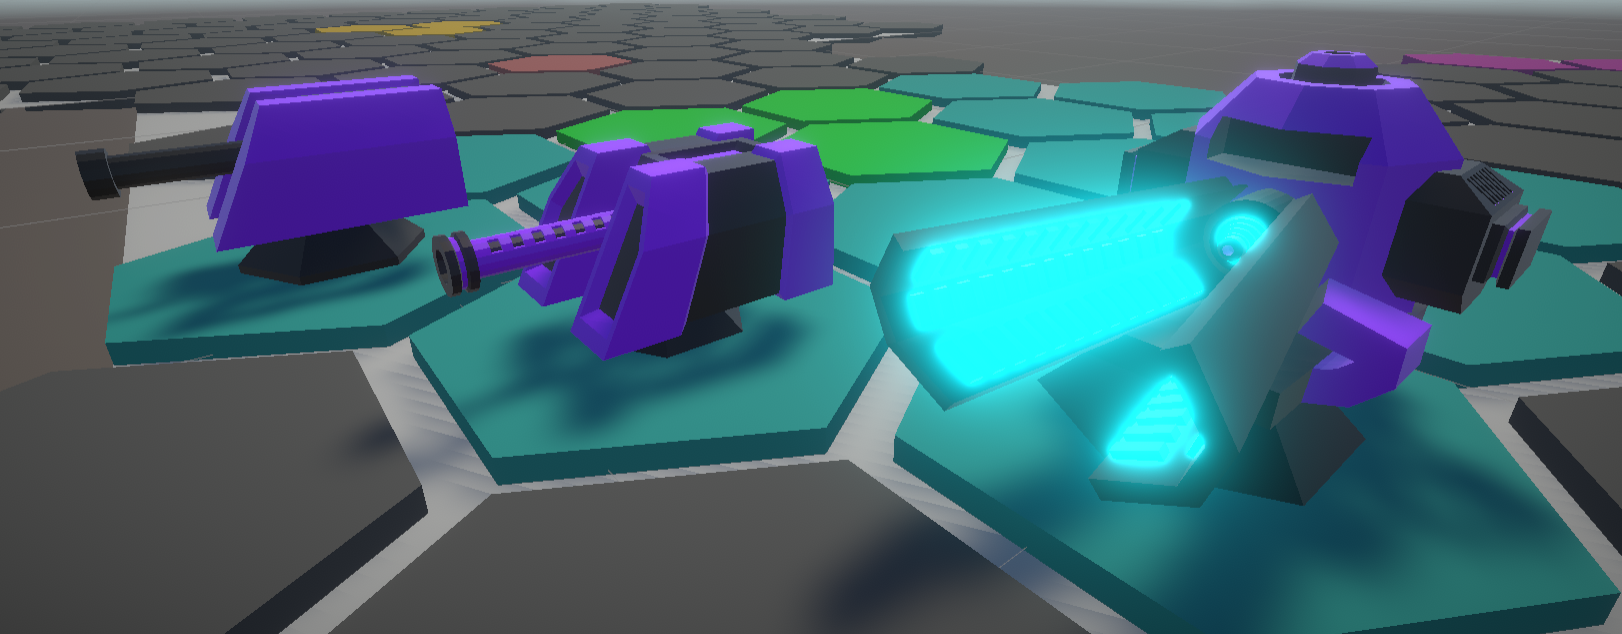
\includegraphics[width=1\textwidth]{railgun.png}
		\caption{Laser}
		\label{fig: railgun}
	\end{figure}

	\begin{figure}[H]
		\centering
		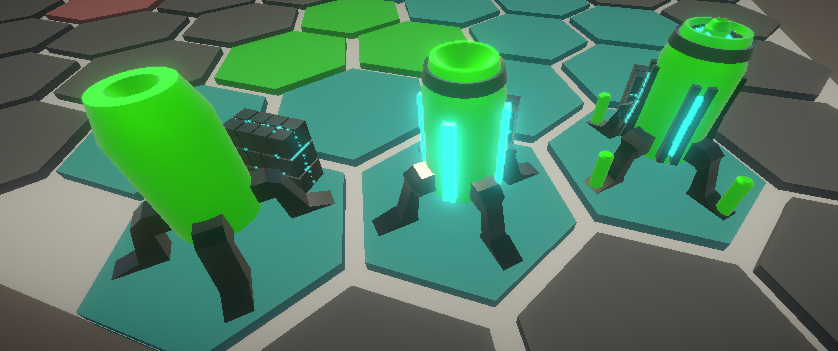
\includegraphics[width=1\textwidth]{excavator.png}
		\caption{Excavator}
		\label{fig: excavator}
	\end{figure}
	
	
	\subsection{Sistemele Jocului}
	
	\subsubsection{Harta de joc}
	
	Pe hara jocului vor fi generate automat obiecte hexagonale. Aceste obiecte pot fi de mai multe tipuri:
	\begin{itemize}
		\item Hexagoane goale (cele gri din (fig: \ref{fig: gridSystem})).
		\item Hexagoane pe care putem construii turnuri de atac. (cele albastre din (fig: \ref{fig: gridSystem}))
		\item Hexagoane pe care putem construii turnul de extragere de resurse. (cele verzi din (fig: \ref{fig: gridSystem}))
		\item Hexagonul pe care va incepe si se va afla comandantul. (cel roz din (fig: \ref{fig: gridSystem}))
		\item Hexagoanele bazei. Baza va ocupa 3 hexagoane de acest tip. (cele galbene din (fig: \ref{fig: gridSystem}))
		\item Hexagonul ocupat. Fiecare hexagon care este ocupat de o anumita structura devine un astfel de hexagon. (are culoarea rosie)
	\end{itemize}

	Inamicii vor calcula drumul pe care merg in functie de toate aceste tipuri de hexagoane. Din acest motiv este nevoie si de cel gol.
	
	\begin{figure}[H]
		\centering
		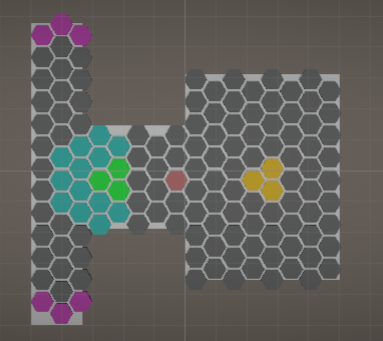
\includegraphics[width=1\textwidth]{grid.png}
		\caption{Harta de joc}
		\label{fig: gridSystem}
	\end{figure}


	
	\subsubsection{Sistemul Turnurilor}
	
	Turnurile pot fi plasate doar pe hexagoanele de constructie. Odata plasate, acestea nu pot fi mutate. Singurele metode de a goli acel hexagon sunt sa fie distrus de un inamic sau sa vindem tureta respectiva. Daca vindem o tureta, vom primii inapoi o parte din banii investiti, bani cu care putem sa imbunatatim turnurile. Toate turnurile au urmatoarele proprietati:
	\begin{itemize}
		\item Viteza de atac
		\item Putere de atac
		\item Viata
		\item Raza de atac
		\item Inamicii pe care pot sa ii atace
	\end{itemize}

	Daca viata turetei ajunge la 0, va fi distrusa automat. Atata timp cat o tureta nu este distrusa, o putem repara, dar reparatiile vor fi executate intr-un anumit timp, iar in acest timp, tureta nu va putea sa atace dar poate sa fie atacata in continuare.
	
	\subsubsection{Comandantul}
	
	Comandantul poate fi mutat pe orice hexagon care nu este deja ocupat. Dupa ce ai ales un hexagon, acesta va incepe sa se miste catre acesta. Cat timp este in miscare, nu poate ataca inamicii. Destinatia poate fi schimbata doar dupa ce a ajuns la destinatie. Are raza medie, rata de atac medie, putere de atac mediu si poate ataca orice tip de inamic.
	
	Acesta poate intra si in turete, imbunatatindu-le exponential.
	
	\subsubsection{Valul de inamici}
	
	Jocul va avea mai multe nivele, care pot fi selectate dintr-un meniu, acestea fiind cat mai diversificate posibil. Inamicii au mai multe puncte din care pot sa vina in functie de nivelul ales. Acestia vin in grupuri de inamici. Intre fiecare grup exista o perioada de repaus in care jucatorul isi poate repara turnurile. In caz ca nu are nevoie de reparatii, poate selecta sa sara peste perioada de repaus, astfel primind bani extra.
	
	
	
	\subsubsection{Nivelele jocului}
	
	Nivelul este terminat cand toti inamicii au fost omorati. Fiecare nivel va avea un scor de maxim 3 stele, care specifica cat de bine s-a descurcat la acest nivel. Scorul este calculat in functie de viata ramasa a bazei la finalul nivelului. Fiecare stea castigata va da bani extra, bani care pot fi folositi in magazinul de imbunatatiri permanente, despre care vom discuta in scurt timp.
	
	Jucatorul poate sa joace din nou nivelele, dar nu va mai primii atat de multi bani ca prima data. Acesta va castiga bani extra de pe stelele castigate doar daca a primit mai multe stele decat turele anterioare.
	
	
	
	\subsubsection{Lock-on}
	
	Jucatorul poate sa apese pe inamici, astfel setand acel inamic drept o prioritate. Fiecare turn care poate ataca acest tip de inamic il va prioritiza fata de alti inamici. De indata ce este omorat, se pierde aceasta prioritate.
	
	
	
	\subsubsection{Magazinul de imbunatatiri permanente}
	
	Intre nivele putem sa cumparat piese de schimb pentru turnurile noastre pentru a le face mai puternice. Aceste piese se pot cumpara doar cu banii castigati de pe urma nivelelor. Imbunatatirile pt fiecare tureta in parte sunt urmatoarele:
	
	\begin{itemize}
		\item Mitraliera automata: atac mai puternic, raza de atac mai mare, costuri mai mici.
		\item Gardul electric: mai multa viata, atac mai puternic, costuri mai mici.
		\item Vulkan: atac mai puternic, range mai mare, atac mai rapid
		\item Aruncatorul de flacari: atac mai puternic, range mai mare
		\item Laser: atac mai puternic, range mai mare
		\item Excavator: da bani mai multi, timpul intre livrarile de bani mai scurt
	\end{itemize}
	
	Fiecare imbunatatire va avea mai multe nivele, fiecare costand din ce in ce mai multi bani, dar vor avea un nivel maxim la care putem duce aceste imbunatatiri.
	
	
	
	\subsubsection{Raid system}
	
	Cand un jucator alege acest mod, este dus la o pagina de login in care trebuie sa isi specifice numele sau sa il lase pe cel generat automat. Dupa ce intra in cont, trebuie sa intre intr-un lobby. Ca sa intre intr-unlobby poate sa creeze el un lobby, sa aleaga un lobby dintr-o lista cu toate lobby-urile existente sau sa intre automat intr-un lobby existent. In cazul ultimei optiuni, in caz ca nu exista nici un lobby, acesta se creeaza automat. La aceasta pagina poate sa selecteze dificultatea nivelului si daca coechipierul este pregatit. De indata ce amandoi jucatorii sunt gata, pot sa inceapta nivelul.
	
	In centrul mapei se afla un monstru imens de foc. Scopul nivelului este sa invingi monstrul impreuna cu coechipierul tau, inainte ca monstrul sa distruga baza vreunuia dintre jucatori.

	Fiecare jucator poate plasa turnuri oriunde, putand sa imbunatateasca, repare sau vinde doar turnurile construite de ei. Amandoi playerii au caracterele lor comandant, dar acestia nu pot intra in aceeasi tureta in acelasi timp. Pentru sistemul de lock-on, doar turnurile jucatorului care a setat lock-on-ul va ataca inamicul prioritizat.
	
	\subsubsection{Atacurile monstrului de foc}
	
	Monstrul de foc are o serie de atacuri predefinite care devin mai puternice in dificultatile avansate.
	
	\begin{itemize}
		\item Abilitate automata: creste puterea de atac pe masura ce pierde din viata
		\item Ploaia de meteoriti: ridica o mana sus si genereaza meteoriti unul dupa altul. Fiecare meteorit cand este construit complet alege un turn si porneste catre directia acestuia. Cand se izbeste de turn explodeaza si scade din viata turnului in functie de dificultatea selectata.
		\item Gheara invartitoare: se invarte 360 grade si loveste toate turnurile de pe harta cu mana lui dreapta.
		\item Meteoritul suprem: cand ajunge la un anumit procentaj de viata incepe acest atac. Alege una dintre bazele jucatorilor (in caz ca sunt mai multi), se roteste spre ea si incepe sa incarce un meteorit imens. Incarcarea acestuia dureaza 30 de secunde. Daca in acest timp jucatorul reuseste sa ii scada suficient de mult viata monstrului, atacul este intrerupt si el devine confuz timp de 10 secunde, timp in care poate fi atacat neintrerupt. Daca jucatorii nu reusesc sa ii scada suficient de mult viata, va lovii puternic cu meteoritul baza selectata si turetele de prin jur.
	\end{itemize}

	Toate interactiunile acestui nivel sunt sincronizate in retea prin utilizarea Photon Engine-ului.
	
	
	\subsection{Analiza proiectului din punctul de vedere al consumatorilor}
	
	\subsubsection{Dificultatea jocului}
	
	Jocul va fi relativ dificil. Jucatorul trebuie sa se gandesca unde sa construiesca anumite turnuri pentru a folosi resursele cat mai bine. La inceput jocul va fi usor, dar pe masura ce progreseaza, nivelele vor devenii din ce in ce mai dificile. Trebuie sa se gandesca si daca poate rezista sa sara peste perioada de repaus intre grupurile de inamici.
	
	Raid system-ul are un nivel de dificultate cu mult mai ridicat, pentru ca trebuie sa se gandeasca cum sa se coordoneze cat mai bine cu coechipierul.
	
	
	
	\subsubsection{Elemente de dependenta}
	
	In caz ca nu putem depasii un anumit nivel, putem juca nivelele anterioare si sa ne asiguram ca luam 3 stele la fiecare nivel. Aceasta metoda de a obtine 3 stele la fiecare nivel poate fi unul din motivele care ii determina pe jucatori sa continue sa joace jocul. Un alt factor ar putea fi sistemul de imbunatatiri permanente.
	
	
	
	\subsubsection{Grupele de varsta vizate}
	
	Acest joc nu are limitari de varsta, poate fi jucat de oricine, dar va fi apreciat cel mai mult de copii si de adolescentii care cauta provocari in jocurile de strategie. Jocul este in principiu facut pentru "casual gamers".
	
	
	
	\section{Implementare proiect}
	
	\subsection{Scena de lupta}
	
	\subsubsection{Initializarea scripturilor}
	\label{section: initialization}
	
	In Unity scripturile au cateva metode care ajuta la initializare.
	
	\textbf{Awake} este metoda care este apelata la inceputul programului si inainte de restul metodelor.
	
	\textbf{Start} este metoda care este apelata dupa ce au fost apelate metodele "Awake" de la toate scripturile.
	
	\textbf{Update} este apelat la fiecare cadru al jocului, aici intervenind o mare parte din logica jocurilor. Apelarea update-ului incepe dupa ce toate metodele "Start" au fost apelate.
	
	Pentru "Start" si "Awake", unity decide automat in ce ordine sa le apeleze, fara ca noi sa putem controla acest lucru. In multe proiecte mai complexe se ajunge in momentul in care, pentru initializatea anumitor sisteme este necesar ca alte sisteme sa fie deja initializate. Cum nu putem controla ordinea de initializare, se ajunge in punctul in care putem primi erori aleatorii din cauza initializarii haotice.
	
	Pentru a combate acest lucru, m-am gandit la un sistem care va permite controlarea initializarii tuturor acestor procese cu usurinta.
	
	\begin{figure}[H]
		\centering
		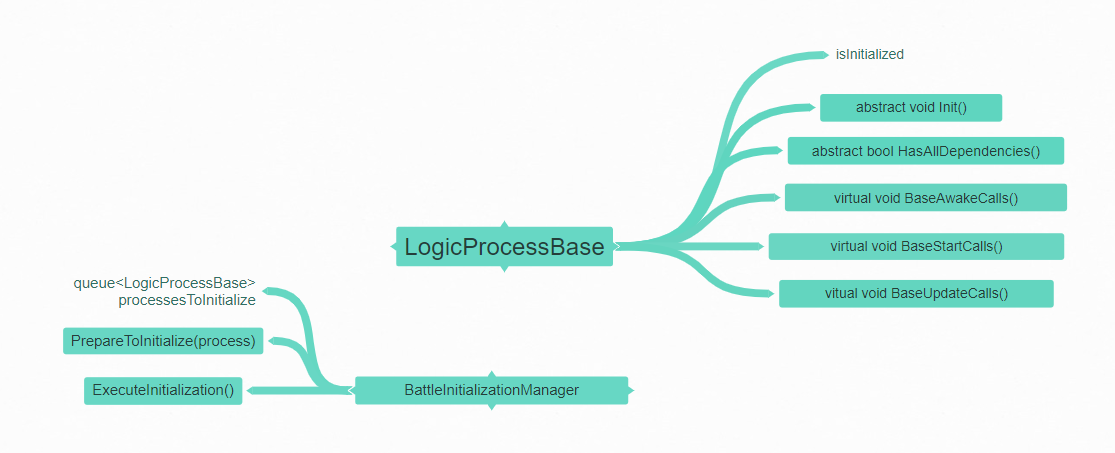
\includegraphics[width=1\textwidth]{logicProcessCoggle.png}
		\caption{Initializarea scripturilor}
		\label{fig: logicProcessCoggle}
	\end{figure}
	
	Am creat clasa LogicProcessBase care ajuta in acest proces. Fiecare script care necesita o initializare mai organizata trebuie sa o mosteneasca. Aceasta contine:
	\begin{itemize}
		\item \textbf{isInitialized} care specifica daca scriptul curent a fost initializat sau nu inca
		\item \textbf{Init()}. In aceasta metoda trebuie sa scriem tot codul de initializare a clasei care mosteneste.
		\item \textbf{HasAllDependencied()}. Este o metoda care returneaza un boolean. In aceasta clasa trebuie sa punem toate dependintele de care are nevoie clasa care mosteneste.
		\item \textbf{BaseAwakeCalls()}. In aceasta metoda apelam "PrepareToInitialize()" din clasa "BattleInitializationManager", despre care vom vorbi in scurt timp.
		\item \textbf{BaseStartCalls()} si \textbf{BaseUpdateCalls()} sunt metode in care trebuie sa scriem tot codul care normal ar fi venit in Start/Update. In unity, nu putem defini Start/Update drept virtual si sa modificam functiile lor pe urma, din acest motiv tot codul din clasele dintr-o ierarhie mai complexa trebuie sa fie scris in aceste metode, iar in clasa cel mai jos din ierarhie trebuie sa le apelam in Awake/Start/Update.
	\end{itemize}

	\textbf{BattleInitializationManager} este a doua clasa de care avem nevoie. Ea este responsabila pentru a executa initializarea propriuzisa a proceselor. 
	
	\textbf{PrepareToInitialize()} este apelata de fiecare proces in metoda lor de awake, iar aceasta metoda va adauga procesul intr-o coada.
	
	\textbf{ExecuteInitialization()} parcurge toate procesele din coada si verifica daca acestea pot fi initializate, apeland "HasAllDependencies()". Daca procesul curent poate fi initializat, atunci apeleaza metoda "Init()" si seteaza "isInitialized = true". Daca nu il poate initializa, il adauga la finalul cozii pentru a fi initializat la final. Acest proces se repeta pana cand coada este goala sau s-a parcurs o data coada cap-coada si nu s-a initializat nici un proces. In acest caz inseamna ca aveau dependinte circulare si oprim procesul de initializare, afisand un mesaj de eroare. Aceasta metoda trebuie apelata in Awake, Start si Update, deoarece, pe parcurs pot aparea noi procese care trebuie initializate, iar programul trebuie sa poata sa detecteze astfel de cazuri.
	
	\subsubsection{Procesarea comenzilor venite de la utilizator}
	
	O alta problema des intampinata in proiectele mari este procesarea comenzilor venite de la utilizator. In cazul in care procesam comenzile in mai multe script-uri, cand vrem sa schimbam modul in care functioneaza comenzile sau sa schimbam platforma pe care ruleaza jocul, va trebuii sa schimbam toate scripturile in care procesam comenzile utilizatorului. In proiectele mari, acest lucru duce la mult timp pierdut si din acest motiv m-am gandit la o metoda cum sa imi organizez mai bine acest sistem.
	
	Ideea propusa de mine este sa pastram toata procesarea de comenzi ale utilizatorului intr-un singur script. Acest script are definite evenimente/delegate pentru toate tipurile de input specifice. Alte scripturi se pot abona la aceste evenimente, iar cand utilizatorul apasa tasta respectiva, toate metodele abonate la evenimentul respectiv vor fi apelate.
	
	Pe langa asta, este necesar sa stim si anumite informatii legate de comanda primita la utilizator. Informatiile aditionale de care am avut nevoie sunt:
	
	\begin{itemize}
		\item Pozitia pe ecran la care a fost apasat mouse-ul/ecranul (in cazul rularii pe android)
		\item Pozitia pe ecran la care a fost ridicata apasarea mouse-ului/ecranului (in cazul rularii pe android)
		\item Daca in clipa curenta este sau nu apasat mouse-ul/ecranul
		\item Timpul la care a fost apasat mouse-ul/ecranul
		\item Timpul la care a fost ridicata apasarea mouse-ului/ecranului
		\item Obiectul pe care utilizatorul a dat click in scena. In momentul cand apasam click, se creeaza un Raycast care are ca origine pozitia mouse-ului pe ecran si care se indreapta catre scena in perspectiva in care se afla camera la clipa curenta. Acest Raycast detecteaza daca a fost lovit un obiect, si daca da, retinem care obiect a fost lovit pt ca alte scripturi sa se poata folosi de aceasta informatie.
		\item Elementul cel mai de sus din ierarhia obiectului lovit. Datorita faptului ca anumite modele au o structura complexa, uneori nu ne este deloc util sa stim in mod direct ce obiect a fost lovit. De exemplu in caz ca apasam peste un turn si Raycast-ul loveste pusca turnului, nu ne va ajuta deloc in cazul in care ne intereseaza sa aflam ce tip de turn am lovit. Din acest motiv, in clipa in care gasim obiectul pe care am dat click, retinem si parintele cel mai de sus din ierarhie.
	\end{itemize}

	Aceasta organizare a procesarii comenzilor ne permite sa schimab tastele folosite cu usurinta si sa adaugam suport pentru dispozitive noi foarte usor. In cazul dispozitivelor noi, putem folosi directive de unity pentru a separa codul specific pentru calculator de cel specific pentru android sau orice alt dispozitiv. Procesarea comenzilor in cele 2 cazuri vor fi diferite, dar datorita faptului ca se invoca evenimentele deja devinite, alte script-uri nu trebuie modificate absolut deloc.
	
	\subsubsection{Grid system}
	
	\subsubsection{Sistemul de navigare}
	
	Caracterele jocului trebuie sa stie pe unde pot sa mearga ca sa ajunga la o anumita destinatie. In acest scop a trebuit sa aleg un algoritm care sa gaseasca cel mai scurt drum posibil. Am avut de ales intre mai multi algoritmi specifici, precum: Dijkstra, A*, Floyd-Warshall, etc.
	
	In cele din urma am ales sa folosesc Floyd-Wharshall. Acest algoritm are complexitatea $O(n^3)$ si presupune construirea celor mai scurte drumuri posibile pornind de la oricare nod catre oricare alt nod din retea. Deoarece construirea drumului se realizeaza doar la inceputul jocului si reconstruirea acestui drum se realizeaza aproape instantaneu, am ales sa folosesc acest algoritm.
	
	"Consideram reteaua orientata $G = (N, A, b)$ reprezentata prin matricea valoare adiacenta $B = (b_{ij}), i, j \in N$ cu
	
	\begin{equation*}
		b_{ij} = \begin{cases}
			b(i, j) \quad daca \quad i \neq j \quad si \quad (i, j) \in A; \\
			0 \quad daca \quad i = j; \\
			\infty \quad daca \quad i \neq j \quad si \quad (i, j) \neq A.
		\end{cases}
	\end{equation*}

	Algoritmul Floyd-Warshall determina matricea distantelor $D = (d_{ij}), i, j \in N$ si matricea predecesor $P = (p_{ij}), i, j \in N$." \cite{grafuriAnul2}
	
	\begin{algorithmic}
		\Function{Floyd-Warshall}{}
			\For{i $\gets$ 1 to n}
				\For{j $\gets$ 1 to n}
					\State $d_{ij} \gets b_{ij};$
					\If{i $\neq$ j and $d_{ij} < \infty$}
						\State $p_{ij} = i;$
					\Else
						\State $p_{ij} = 0;$
					\EndIf
				\EndFor
			\EndFor
			
			\For{k $\gets$ 1 to n}
				\For{i $\gets$ 1 to n}
					\For{j $\gets$ 1 to n}
						\If{$d_{ik} + d_{kj} < d_{ij}$}
							\State $d_{ij} = d_{ik} + d_{kj};$
							\State $p_{ij} = p_{kj};$
						\EndIf
					\EndFor
				\EndFor
			\EndFor
		\EndFunction
	\end{algorithmic}

	\begin{algorithmic}
		\Function{Reconstruire Drum}{}
			\State k = n;
			\State $x_k = j$
			\While{$x_k \neq i$}
				\State $x_{k - 1} = p_{ix_k};$
				\State k = k - 1
			\EndWhile
		\EndFunction
	\end{algorithmic}

	Drumul minim este $D_{ijp} = (x_k, x_{k+1}, \dots, x_{n-1}, x_n) = (i, x_{k+1}, \dots, x_{n-1}, j)$
	
	\subsubsection{Interfete folosite}
	
	Pentru ca o serie de obiecte din joc trebuie sa urmeze aceleasi concepte, am decis sa ma folosesc de interfete pentru a le definii modul in care trebuie sa functioneze. 
	\newline
	
	\textbf{IMovable}
	
	Deoarece inamicii si comandantul se pot misca pe mapa, am definit aceasta interfata pentru a defini aceleasi concepte pentru toate caracterele care au nevoie de a se misca pe mapa. Interfata se foloseste de sistemul de navigare definit anterior si contine urmatoarele:
	
	\begin{itemize}
		\item Nodul curent la care se afla
		\item Nodul destinatie
		\item Nodul urmator la care trebuie sa se mute ca sa se apropie de destinatie
		\item Viteza de deplasare
		\item Distanta fata de urmatorul nod pt care consideram ca am ajuns la acesta. Deoarece lucram cu obiecte in spatiu 3D, este nevoide de o asemenea valoare.
		\item Un boolean care defineste daca am ajuns sau nu la destinatie
		\item O metoda care seteaza nodul urmator la care trebuie sa ajungem ca sa ne apropiem de destinatie. Acesta face apel la matricea construita de sistemul de navigare.
		\item O metoda care misca propriuzis obiectul catre urmatorul nod
		\item O functie care verifica daca am ajuns sau nu la destinatie.
	\end{itemize}
	\bigskip


	\textbf{IAttacker}
	
	 Este o interfata pe care toate obiectele/caracterele care vor sa atace alte obiecte trebuie sa o mostendeasca. Aceasta contine urmatoarele:
	 
	 \begin{itemize}
	 	\item Obiectul pe care trebuie sa il atace. Tipul este definit la mostenirea clasei datorita sablonului definit pentru interfata.
	 	\item Puterea de atac
	 	\item Raza de atac
	 	\item Durata intre atacuri
	 	\item Timpul la care s-a executat ultimul atac
	 	\item Intervalul de timp intre care se cauta un nou inamic
	 	\item Metoda care afisaza/ascunde raza obiectelor din scena. Raza acestora a fost defnita intr-un shader special creat in Shader Graph
	 	\item O metoda care cauta cel mai apropiat inamic daca exista in raza
	 	\item Metoda de atac pe care fiecare obiect o implementeaza diferit.
	\end{itemize}
 	\bigskip
 	
 	\textbf{IDestroyable}
 	
 	Fiecare obiect care are o viata anume si care poate fi distrus trebuie sa mosteneasca aceasta interfata. Aceasta contine urmatoarele:
 	
 	\begin{itemize}
 		\item Viata obiectului.
 		\item Banii primiti cand obiectul este distrus
 		\item O metoda care distruge obiectul respectiv cand viata lui a ajuns la 0
 	\end{itemize}
 	\bigskip
 	
 	\textbf{IRecoverable}
 	
 	Turnurile pot sa isi refaca viata, iar ca un concept pentru viitor, ar putea sa existe si anumiti inamici care refac viata altor inamici. Interfata contine urmatoarele:
 	
 	\begin{itemize}
 		\item Cata viata se reface in fiecare secunda cand efectul este aplicat.
 		\item Costul refacerii in cazul in care este de dorit un cost.
 		\item Un boolean care verifica daca se reface sau nu in clipa curenta.
 		\item O metoda care porneste procesul de refacere
 	\end{itemize}
	
	\subsubsection{Ierarhia inamicilor}
	
	\begin{figure}[H]
		\centering
		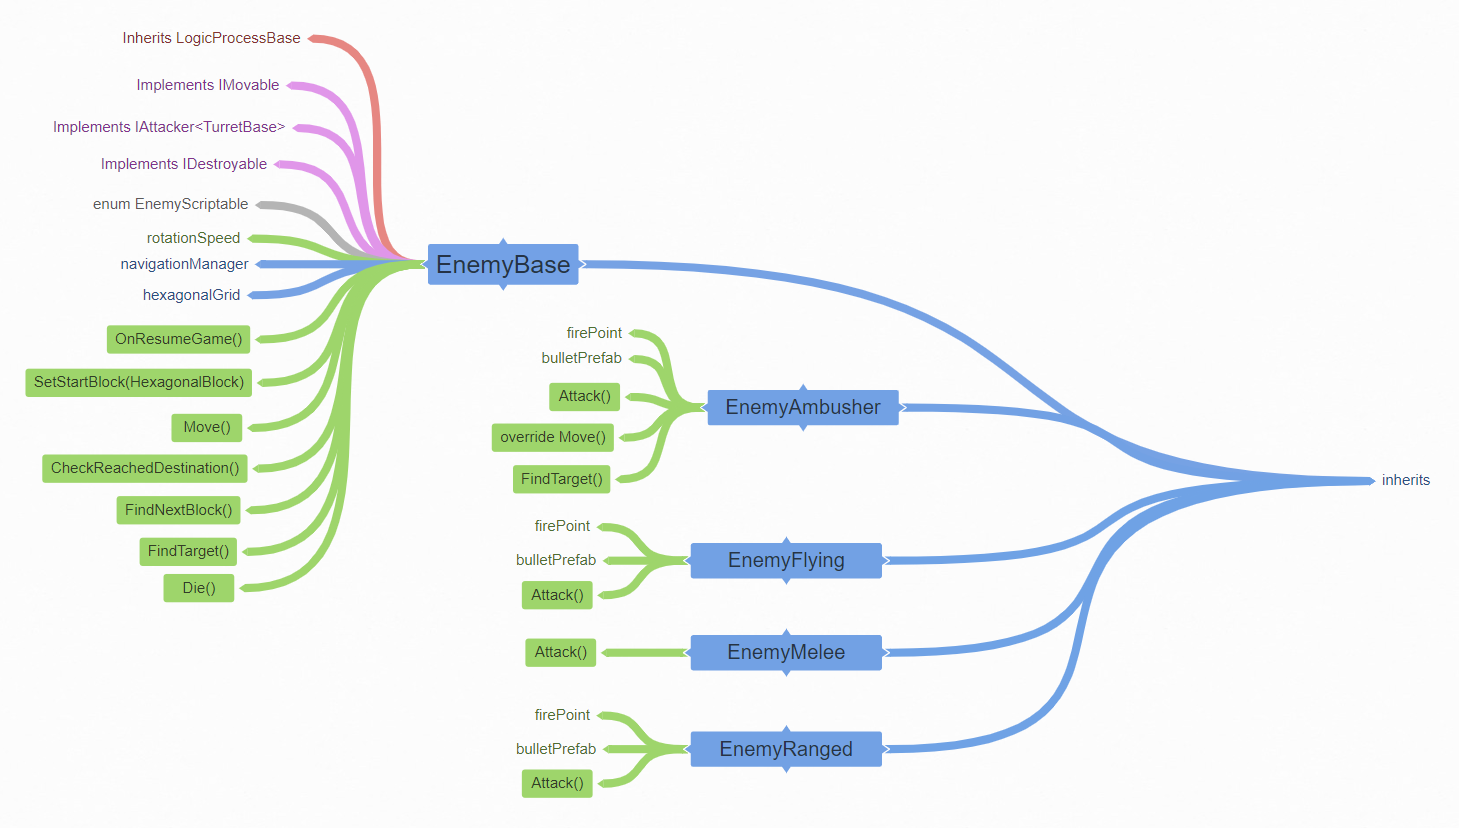
\includegraphics[width=1\textwidth]{EnemyHierarchy.png}
		\caption{Ierarhia inamicilor}
		\label{fig: enemyHierarchy}
	\end{figure}

	In \ref{fig: enemyHierarchy} am definit intr-un mod simplu si colorat modul in care trebuie structurata ierarhia inamicilor din joc.
	
	Clasa EnemyBase este clasa parinte care defineste modul principal in care inamicii trebuie sa functioneze. Aceasta clasa implementeaza 3 interfete utile, si anume IMovable, IDestroyable si IAttacker<TurretBase>. Precum am explicat si anterior, interfata IAttacker defineste un sablon care specifica tipul de obiect pe care poate sa il atace, in cazul nostru, clasa TurretBase care va fi explicata in urmatoarea sectiune.
	
	Aceasta clasa face referire si la sistemul ne navigare si la sistemul hartii hexagonale, si din acest motiv este nevoie sa isi faca initializarea doar dupa ce aceste doua sisteme si-au terminat initializarea lor. In acest scop, putem sa mostenim clasa LogicProcessBase, care a fost descrisa in capitolul \ref{section: initialization}.
	
	Functiile implementate de aceasta clasa sunt in mare parte functiile mostenite dupa implementarile interfetelor descrie, cu cateva exceptii referitoare la alte sisteme din joc. Un astfel de sistem este cel de a pune pe pauza jocul. Can jocul este pus pe pauza, toate scripturile care se foloseau de timpul actual al jocului nu vor actiona in modul asteptat dupa ce reluam jocul. Din acest motiv este nevoie sa implementam functia OnResumeGame() care va fi apelata cand se reia jocul, iar in aceasta functie trebuie sa setam toti temporizatorii din script la valorile necesare.
	
	Aceasta clasa nu este suficienta pentru a definii toate tipurile de inamici, deoarece face dificila diferentierea intre inamici pentru anumite sisteme si anumiti inamici actioneaza diferit fata de standard. Din acest motiv este necesar sa definim o serie de clase pentru fiecare inamic in parte, care sa mosteneasca aceasta clasa de baza, si care sa isi adauge propia lor logica la standardul definit de EnemyBase.
	
	\textbf{EnemyAmbusher} nu se foloseste de sistemul de navigare. Este inamicul bombardier, care zboara prin aer direct catre baza jucatorului. Cand ajunge in contact cu aceasta, lanseaza bombe care provoaca multe pagube, dupa care isi continua drumul, parasind scena de lupa. Din acest motiv metodele Move() si FindTarget() trebuie sa fie suprascrise.
	
	\textbf{EnemyFlying} si \textbf{EnemyRanged} sunt inamici care urmeaza in totalitate logica definita de EnemyBase. Singura exceptie la aceste doua clase este ca anumite turnuri vor face diferentiere intre ele. O parte din turnuri pot sa atace doar inamicii de sol (EnemyRanged si EnemyMelee) iar alte turnuri pot sa atace doar inamicii zburatori (EnemyFlying si EnemyAmbusher).
	
	\textbf{EnemyMelee} este un inamic care sa atace alte turnuri doar cand a ajuns langa turnuri. Din acest motiv metoda lui de atac trebuie sa fie suprascrisa putin.
	
	\subsubsection{Ierarhia turnurilor defensive}
	
	Ierarhia turnurilor este putin mai complexa si va fi descrisa pe bucati.
	
	\ \\
	\textbf{TurretBase}
	
	Urmand aceeasi logica ca la inamici, am definit o clasa de baza pentru modul in care trebuie sa actioneze un turn defensiv. Acesta implementeaza doua interfete: IDestroyable si IAttacker<EnemyBase>. Sablonul de la IAttacker defineste faptul ca un turn defensiv poate sa atace obiecte de tipul EnemyBase, care este clasa din care mostenesc toti inamicii jocului.
	
	TurretBase are si ea nevoie de o initializare controlata si din acest motiv trebuie sa mosteneasca clasa LogicProcessBase. TurretBase defineste proprietatile turnurilor, cum ar fi viata, puterea de atac, etc. Pe langa asta, majoritatea turnurilor pot fi imbunatatine, proprietatile crescand exponential cand acest lucru se intampla. Din acest motiv a fost nevoie sa creez fisiere configurabile care definesc valori pt proprietatile turnurilor. Aceasta clasa detine o instanta a unui astfel de fisier, si defineste o functie "SetLevelProp(int level)" care citeste fisierul configurabil si seteaza toate proprietatile in functie de acesta. Pe langa asta, cand turnurile sunt imbunatatite, le schimba modelul 3D pentru a avea o schimbare vizuala.
	
	Clasa defineste si alte metode care au fost abordate in capitolele anterioare, precum: Die(), OnResumeGame(), Init(), etc. Functia DrawRange() afiseaza/ascunde raza de atac a turnului, raza care a fost construita intr-un shader special definit in Shader Graph.
	
	\ \\
	\textbf{PlayerBase}
	
	PlayerBase este o clasa care mosteneste TurretBase, si reprezinta baza de operatii a jucatorului. Aceasta implementeaza o parte din actiunile definite in interfete, precum: Attack(), FindTarget(), etc.
	
	Pe langa asta, cand baza jucatorului ramane fara viata si este distrusa, jocul trebuie sa se termine. Acest lucru poate fi realizat foarte usor prin suprascrierea metodei Die(). Cand baza ramane fara viata, instiinteaza managerul jocului, iar pe urma acesta isi porneste procesul de incheiere al nivelului. Mai multe detalii vor fi discutate in capitolul \ref{section: gameState}
	
	\ \\
	\textbf{BuildableTurret}
	
	BuildableTurret este clasa care mosteneste TurretBase si defineste functionalitatea pentru toate turnurile care pot fi construite pe harta de joc. Aceasta clasa implementeaza IRecoverable, care defineste modul in care turnurile pot sa isi refaca viata. De indata ce turnul a fost lovit de un inamic, se calculeaza un cost necesar pentru a readuce turnul la viata maxima. In caz ca jucatorul are suficienti bani si doreste sa refaca turnul, acesta va incepe procesul refacere. Pe parcursul catorva secunde, se va reface treptat pentru viata lipsa in momentul inceperii acestui proces. In acest timp turnul nu poate sa atace inamicii, dar poate sa fie lovit in continuare de acestia, deci nu este garantat ca va revenii la viata maxima dupa terminarea procesului.
	
	O alta functionalitate majora a turnurilor este optiunea de a inbunatatii turnurile. Cand utilizatorul selecteaza un turn, se cauta in fisierul configurabil costul necesar pentru a imbunatatii turnul la nivelul urmator, in caz ca nu a ajuns inca la nivelul maxim. In caz ca jucatorul are suficienti bani se apeleaza metoda Upgrade(), care verifica daca s-a ajuns la nivelul maxim si daca nu, dezactiveaza toate starile defavorabile ale turnului (cum ar fi raza turnului), creste nivelul si apeleaza metoda SetLevelProp() pentru a citi din nou fisierul de configuratie pentru nivelul nou.
	
	Turnul poate fi vantut de jucator in caz ca este in criza de bani sau vrea sa mute turnul in alta locatie. In acest caz se calculeaza banii pe care ii primeste jucatorul, se dezaciveaza toate starile si functionalitatile turnului si se distrug referintele specifice. Tote acestea se intampla in metoda SellTurret() implementata in aceasta clasa.
	
	Ultima functionalitate adaugata de aceasta clasa este cea de a permite turnului sa fie controlat de comandantul jocului. Aceasta functionalitate va fi descria in detaliu in sectiunea \ref{section: commander} 
	
	\ \\
	\textbf{Turnurile specifice}
	
	Cel mai jos nivel din ierarhie presupune definirea claselor specifice pentru fiecare tip de turn in parte, fiecare dintre acestea mostenind clasa BuildableTurret si adaugand/modificand logica stabilita pana in acest punct in functie de caz.
	
	\begin{itemize}
		\item \textbf{TurretElectricFence}. Este turnul care are viata foarte mare dar raza de atac foarte mica. Poate sa atace doar inamicii de lupta apropiata si actioneaza drept un zid care pazeste toate celelalte turnuri de atacurile inamicilor. Aceast turn modifica functionalitatea prin care se gaseste ce inamic trebuie sa atace si modul in care ataca inamicul.
		\item \textbf{TurretExcavator}. Acest turn este cel mai diferit de norma, in sensul in care nu poate ataca deloc inamicii. Este un turn care la un anumit interval de timp farmeaza resurse, pe care le converteste la bani de joc. Din acest motiv a fost nevoie sa scape complet de cautarea inamicilor, iar metoda de atac a suprascris-o in functionalitatea de farmare de bani.
		\item \textbf{TurretFlamethrower}. De indata ce un inamic intra in raza acestui turn, lanseaza flacari violente in directia inamicului, flacari care ranesc toti inamicii care stau in ele. Turnul prioritizeaza inamicii de atac de aproape, dar in cazul in care nu exista astfel de inamici, ataca inamicii cu raza de atac. Nu poate sa atace inamicii zburatori sau cei bombardieri.
		\item \textbf{TurretMachineGun}. Este turnul universal care poate sa atace toti inamicii jocului. Acesta lanseaza gloante foarte rapid catre inamici, dar gloantele individual nu provoaca foarte multe daune. Fiecare nivel presupune o viteza de atac mai mare.
		\item \textbf{TurretLaser}. Acest turn ataca inamicii cu un laser foarte puternic care distruge compozitia moleculara a inamicului in fiecare clipa in care acestia sunt in raza turnului. Poate ataca inimacii de atac apropiat si cei de la distanta, dar ii prioritizeaza pe cei de la distanta. Nu poate ataca inamicii zburatori sau pe cei bombardieri.
		\item \textbf{TurretVulkan}. Este turnul special impotriva inamicilor zburatori si a celor bombardieri. Nu poate ataca inamicii de sol, dar in schimb lanseaza rachete catre cei zburatori, rachete care explodeaza cand ajung in contact cu acestia.
	\end{itemize}
	
	\subsubsection{Comandantul}
	\label{section: commander}
	
	Comandantul este un caracter special care poate fi miscat oriunde dorim pe harta si care ataca inamicii din raza lui de atac, cat timp nu se deplaseaza catre o noua locatie.
	
	In acest scop, clasa Commander implementeaza interfetele IMovable si IAttacker<EnemyBase>. Comandantul nu poate sa fie distrus si din acest motiv nu este nevoia implementarii interfetei IDestroyable.
	
	Comandantul are si el un fisier de configurare care specifica statusurile lui, cum ar fi viata, viteza de miscare, puterea de atac, etc. Pentru a se putea deplasa pe harta, are nevoie sa faca referire la sistemul de navigare si la cel al hartii de joc (grid system). Din acest motiv este necesar sa mosteneasca LogicProcessBase, ca sa isi execute initializarea doar dupa celelalte sisteme au reusit sa si-o termine pe a lor.
	
	Majoritatea functiilor sunt similare cu cele ale turnurilor (Attack, DrawRange, FindTarget, etc.) asa ca nu vor fi reluate aici. 
	
	Pe langa aceste functionalitati, comandantul poate sa intre in turnuri si sa le controleze, marindu-le astfel productivitatea. Cand acesta intra in turnuri, le mareste raza, viteza, puterea de atac si in cazul excavatorului de resurse, creste banii primiti la fiecare livrare de resurse. Ca sa poata intra in turnuri, trebuie sa se deplaseze la acel turn la comanda jucatorului, iar cand turnul este distrus/vandut, acesta iese din turn si se misca catre cel mai apropiat nod din graful hartii de joc care nu este deja ocupat. Comandantul poate sa iasa din turn si fara ca acesta sa fie dsitrus, dar acest lucru se intampla numai la comanda jucatorului.
	
	\subsubsection{Controlul turnurilor si starilor de joc}
	\label{section: gameState}
	
	\subsection{Selectarea nivelelor}
	
	\subsubsection{Structura meniului}
	
	\subsubsection{Generarea dinamica a meniului}
	
	
	\subsection{Salvarea datelor}
	
	\subsubsection{Salvarea automata}
	
	\subsubsection{Criptarea si decriptarea datelor}
	
	
	\subsection{Magazinul de imbunatatiri permanente}
	
	\subsubsection{Structura meniului}
	
	\subsubsection{Generarea dinamica a meniului}
	
	
	\subsection{Sistemul co-op}
	
	\subsubsection{Modul de lucru cu Photon Engine}
	
	\subsubsection{Inregistrare si camera de asteptare}
	
	\subsubsection{Sincronizarea datelor}
	
	\subsubsection{Monstrul de foc}
	
	\subsection{Metode de imbunatatire a proiectului}
	
	\subsubsection{Arta imbunatatita}
	
	\subsubsection{O poveste pentru joc}
	
	\subsubsection{Monstrii multipli pentru modul co-op}
	
	\section{Concluzii}
	
	
	\pagebreak
	\begin{thebibliography}{3}
		\bibitem{gameProgrammingComplete} 
		Mike McShaffry, David Graham. \newline
		\textit{Game Coding Complete Fourth Edition}. 2012
		
		\bibitem{bookOfLenses}
		Jesse Schell.  \newline
		\textit{The Art of Game Design: A Book of Lenses 1st Edition}. 2008
		
		\bibitem{grafuriAnul2}
		Eleonor Ciurea, Laura Ciupala.  \newline
		\textit{Algoritmi: Introducere in algoritmica fluxurilor in retele}. 2006
		
	\end{thebibliography}
	
	
\end{document}